\begin{comment}\\
%\newglossaryentry{kiln}
%{
% name=kiln,
%description={German: Brennofen (m.);\\Français: fourneau (m.)},
%plural=kilns
%}

%Make Glossary properly...
%\acrodef{VB}{Visula Basic}
%\makeglossaries
%\newglossaryentry{Availability Zone}
%{
name=Availability Zone,
description={Eine Verfügbarkeitszone ist einfach ein Datenzentrum oder eine Sammlung von Datenzentren. Jede Verfügbarkeitszone in einer Region verfügt über eine separate Stromversorgung, Netzwerk und Konnektivität, um die Gefahr eines gleichzeitigen Ausfalls in beiden Zonen zu verringern \footnote{Vgl. AWS Certified Solutions Architect - Associate (SAA-C02)\cite{AWS1}, S.42}.
  }
}
%\clearpage
\end{comment}
\textbf{Availability Zone}\\
Eine Verfügbarkeitszone ist einfach ein Datenzentrum oder eine Sammlung von Datenzentren. Jede Verfügbarkeitszone in einer Region verfügt über eine separate Stromversorgung, Netzwerk und Konnektivität, um die Gefahr eines gleichzeitigen Ausfalls in beiden Zonen zu verringern \footnote{Vgl. AWS Certified Solutions Architect - Associate (SAA-C02), S.42.\cite{AWS1}}.
\\\\
%\textbf{Auto-Scaling}
%\textbf{Amazon S3}
%\textbf{AWS Lambda-Funktion}
%\textbf{Amazon SNS}
%\textbf{CPU-Auslastung(CPU-Utilization)}
%Eine geringe Auslastung wird von AWS definiert, wenn Instanzen in den letzten 14 Tagen eine CPU-Auslastung von 10% oder weniger hatten und wenn der Netzwerkverkehr in den letzten 4 Tagen gleich oder kleiner als 5 MB war.


\textbf{Buckets}\\
Buckets sind in AWS-S3 Behälter, wo Dateien wie Bilder oder Videos gespeichert werden\footnote{Vgl. AWS: Amazon Simple Storage Service - User Guide. S.4.\cite{AMZ18}}.
\\\\
\textbf{Cloud-Computing}\\
Das NIST definiert Cloud Computing als das Modell zur Ermöglichung eines allgegenwärtigen, bequemen und bedarfsgerechten Netzzugangs zu einem gemeinsamen Pool konfigurierbarer Rechenressourcen (z. B. Netze, Server, Speicher, Anwendungen und Dienste), die mit minimalem Verwaltungsaufwand oder minimaler Interaktion mit dem Dienstanbieter schnell bereitgestellt und freigegeben werden können\footnote{Vgl. The NIST Definition of Cloud Computing. S.6
  \cite{CC1}}.
%Das Cloud-Modell besteht aus fünf wesentlichen Merkmalen, drei Dienstmodellen und vier Bereitstellungsmodellen.
\\\\
\textbf{Cloud-Dienst}\\
Bei Cloud-Dienste geht es um sämtliche
Infrastruktur-Komponenten wie die Server, Rechenleistung, Netzkapazitäten, Kommunikationsgeräte, Speicher, Archivierungs- und Backup-Systeme und andere Komponenten der Rechenzentrum- und Netzinfrastruktur, die von dem Cloud-Service-Provider zur Verfügung gestellt werden. Der Anwender kann über das Netzwerk (i. d. R. Internet) auf die virtuellen Services zugreifen. Beispiele für Cloud-Dienste stellen die Elastic Compute Cloud (EC2) von Amazon, die MicrosoftWindows Azure virtuelle Maschinen und die Google Compute Engine\footnote{Vgl. Helmut Krcmar. (2015). Einsatzfelder und Herausforderungen des Informationsmanagements. Informationsmanagement. 6. Auflage S.724\cite{IM1}}.
\\\\
%\textbf{EC2-Instanz}
\textbf{Instance family}\\
Instanzfamilien sind eine Sammlung von EC2-Instanzen, die nach dem Verhältnis von\\ Speicher, Netzwerkleistung, CPU-Größe und Speicherwerten zueinander gruppiert sind. Zum Beispiel bietet die m4-Familie von EC2 eine ausbalancierte Kombination von Rechen-, Speicher- und Netzwerkressourcen\footnote{Vgl. AWS Certified Solutions Architect - Associate (SAA-C02). S.95\cite{AWS1}}.
\\\\
\textbf{Instagram-Story}\\
Bei Instagram Stories handelt es sich um kurzen visuellen Content in der Regel Bilder oder kurze Videos, die nach 24 Stunden automatisch aus der Applikation Instagram verschwinden(Stand November 2021)\footnote{Vgl. Online Marketing: Definition von Instagram Story? o.S.\cite{IG2}}.
\begin{comment}
\\\\
\textbf{On-Demand}\\
...
horizontale und vertikale Skalierung
\\\\
\textbf{On-Premise}\\
...\\\\
\end{comment}
\textbf{Region}\\
Die Region ist ein völlig unabhängiges und eigenständiges geografisches Gebiet. Jede Region hat mehrere, physisch getrennte und isolierte Standorte, die als Availability Zones bekannt sind. Beispiele für Regionen sind London, Dublin, Sydney, usw \footnote{Vgl. AWS Certified Solutions Architect - Associate (SAA-C02)\cite{AWS1}, S.42}.
\\\\
\textbf{Tag}\\
Ein \textit{Tag} (Markierung) ist eine Markierung, die einer AWS-Ressource zuordnet. Jeder Tag (Markierung) besteht aus einem Schlüssel und einem optionalen Wert\footnote{Vgl. Amazon Elastic Compute Cloud - Benutzerhandbuch für Linux-Instances\cite{AMZ26}, S.1570}.
\begin{figure}[h!]
  \centering
  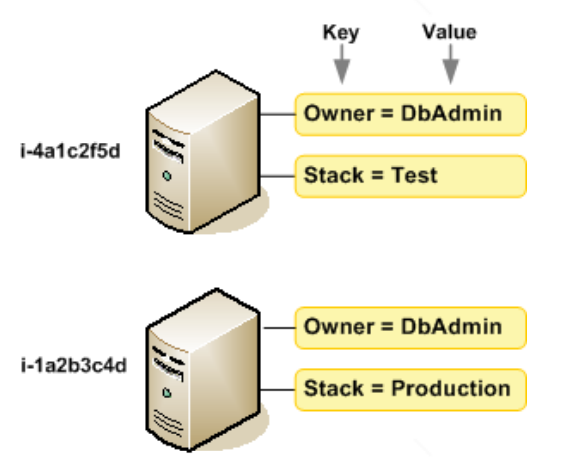
\includegraphics[scale=0.4]{sources/TagExample}
  \caption[Beispiel für ein Tag]{}\label{fig:TagExample}
  Beispiel für ein Tag{\cite{AMZ26}, S.1570}.
\end{figure}
\\\\
\\\\
%PAYG %https://www.nimbix.net/glossary/pay-go
\textbf{Metadaten}\\
Metadaten liefern Informationen über den Inhalt eines bestimmten Objekts. Ein Bild kann beispielsweise Metadaten enthalten, die beschreiben, wie groß das Bild ist, die Farbtiefe, die Bildauflösung, wann das Bild erstellt wurde und andere Daten. Die Metadaten eines Textdokuments können Informationen darüber enthalten, wie lang das Dokument ist, wer der Autor ist, wann das Dokument geschrieben wurde und eine kurze Zusammenfassung des Dokuments\footnote{Vgl. Techterms Definition Metadata\cite{MET}}.
\\\\
%RI-Coverage
%RI-Utilization
\textbf{Startkonfiguration}\\
Eine Startkonfiguration ist eine Instance-Konfigurationsvorlage, die eine Auto-Scaling-Gruppe zum Starten von EC2-Instances verwendet\footnote{Vgl. Amazon EC2 Auto Scaling - Benutzerhandbuch. S.54 \cite{AMZ31}}.
%https://docs.aws.amazon.com/autoscaling/ec2/userguide/create-launch-template.html
\\\\
%\textbf{Scale-In/Out}\\
%\\\\\textit{Scale-Out} genannt und eine für das Verringern von Rechenkapazität bezeichnet als \textit{Scale-In}.
\textbf{Maschinelles Lernen}\\
Maschinelles Lernen ist ein Teilbereich der künstlichen Intelligenz (KI). Beim maschinellen Lernen werden Algorithmen darauf trainiert, Muster und Korrelationen in großen Datensätzen zu finden und auf Basis dieser Analyse die besten Entscheidungen und Vorhersagen zu treffen. Auf diese Weise wird die Rechenkapazität von EC2-Instanzen auf der Grundlage früherer Muster vorhergesagt\footnote{Vgl. SAP: Definition von machinellen Lernen\cite{ML1}}.
\\\\
\textbf{YAML}\\
YAML ist eine benutzerfreundliche Daten-Serialisierungs  Sprache für alle Programmiersprachen\footnote{Vgl. YAML Org: Definition von YAML\cite{YAML}}.
%Governance, Compliance ?
